%\documentclass[a4paper,10pt]{article}
\documentclass{scrartcl}
 \usepackage[T2A]{fontenc}
 \usepackage[utf8]{inputenc}
 \usepackage[english,russian]{babel}
 \usepackage{amsmath}
 \usepackage{amssymb}
 \usepackage{tikz}
 \usepackage{pgfplots}
 \usepackage{comment}


 \DeclareMathOperator{\rot}{rot}
 \DeclareMathOperator{\mdiv}{div}
 \DeclareMathOperator{\RE}{Re}
 \renewcommand{\Re}{\mathop{\mathrm{Re}}\nolimits}
 \DeclareMathOperator*{\argmax}{argmax}

\if 0
%opening
 \title{Численное исследование 3-х мерных не изотермических течений несжимаемой жидкости в прямоугольной каверне с подвижной крышкой}
 \author{Владимир Олегович Пиманов}
 \date{2013 год}
\fi


\begin{document}
%\large
% \maketitle

\thispagestyle{empty}
\begin{center}
{\bfseries МОСКОВСКИЙ ГОСУДАРСТВЕННЫЙ УНИВЕРСИТЕТ им.~М.{\,}В.{\,}Ломоносова}\\
\vspace{2ex}Факультет вычислительной математики и кибернетики \\
\vspace{2ex}Кафедра вычислительных методов \\
\end{center}

\vfill

\begin{center}
{\huge {\bfseries Дипломная работа

\vspace*{1cm}

Численное исследование 3-х мерных не изотермических течений несжимаемой жидкости в прямоугольной каверне с подвижной крышкой} \\[25mm]}

\end{center}

\vfill 

\hspace*{7cm} Выполнил:

\hspace*{7cm} Пиманов Владимир Олегович,

\hspace*{7cm} 505 группа

\hspace*{7cm} Научныe руководители:

\hspace*{7cm} к.ф.м.н. И.{\,}С.{\,}Калачинская,

\hspace*{7cm} кафедра ВМ, ВМК МГУ;

\hspace*{7cm} д.ф.м.н. Н.{\,}В.{\,}Никитин,

\hspace*{7cm} НИИ Механики МГУ

\hspace*{7cm} 

\bigskip

\vfill

\begin{center}
{\bfseries Москва 2013}
\end{center}

\newpage
\tableofcontents
\newpage

\section{Аннотация}
  В дипломной работе исследуется течение вязкой несжимаемой изотермической жидкости в каверне с подвижной крышкой. 
  Движение жидкости описывается системой уравнений Навье-Стокса. Каверна имеет форму траншеи, бесконечно длинной 
  вдоль одного направления, с квадратным поперечным сечением. Известно, что в такой геометрии при небольших числах 
  Рейнольдса у поставленной задачи
  существует устойчивое двумерное стационарное решение, называемое далее \textit{основное течение}. В работе приведены результаты
  расчета основного течения при некоторых числах Рейнольдса. Результат получен прямым численным интегрированием задачи 
  Коши до установления стационарного течения конечно-разностным методом, известным как метод Никитина. 
  На полученное таким образом основное течение наложены малые 
  трехмерные возмущения, и их эволюция исследована в рамках линеаризованной системы уравнений. Решение 
  соответствующей спектральной задачи требует большого объема памяти и возможно лишь при небольших числах Ренольдса.
  В общем случае, эволюция малых возмущений исследовалась прямым численным интегрированием по времени. 
  Соответствующая программа была написанна с применением технологии MPI. Расчет проведен на суперкомпьютере 
  МГУ им М.В.~Ломоносова "Чебышев". Были определены декременты затухания при некоторых числах Рейнольдса и было 
  определено пороговое число Рейнольдса, при котором основное течение теряет устойчивость к малым трехмерным возмущениям. 
  В качестве введения в дипломную работу включена краткая история гидродинамики.

\newpage  
  
  % http://iproc.ru/interesting/hydro-history/1/
% http://iproc.ru/interesting/hydro-history/2/

\section*{Краткая история гидродинамики \cite{history}}

Что же такое гидродинамика? Энциклопедия дает следующее определение~\cite{wiki}:

<<Гидродинамика~--- раздел физики сплошных сред, изучающий движение идеальных и реальных жидкости и газа.
Как и в других разделах физики сплошных сред, прежде всего осуществляется переход от реальной среды, 
состоящей из большого числа отдельных атомов или молекул, к абстрактной сплошной среде, для которой и 
записываются уравнения движения.>>

Следует обратить внимание на то, что гидродинамика, несмотря на свое название («гидро»~--- вода, 
«динамика»~--- движение), изучает не только движение жидкости, но и движение газа, хотя на первый 
взгляд между ними очень много различий.

Помимо гидродинамики есть еще гидростатика, изучающая равновесие жидкостей. Но, в отличии от 
гидродинамики, законы гидростатики (законы Паскаля и Архимеда) просты и не подвергаются сомнению.

Несмотря на простоту законов, описывающих покоящуюся жидкость, движущаяся жидкость долгое время 
оставалась (и всё еще остается) неподвластна умам ученых. Многие ека философы пытались разгадать 
тайны течения воды (самой распространенной жидкости на Земле). Но зарождение гидродинамики как науки 
началось после открытия Ньютоном своих законов, которые стали отправной точкой для математического 
описания движения жидкости.

\subsection*{Ранние попытки исследовать течение жидкости}

О том, как среда сопротивляется движению тела, можно узнать, наблюдая за падением тел в воде или в воздухе. 
Проведением подобных опытов одним из первых занялся Леонардо да Винчи (1452--1519). 
Его дело продолжил другой «шаробросатель»~--- Галилео Галилей (1564--1642). 
Сбрасывая с наклонной Пизанской башни тяжелые и легкие шары, он установил независимость 
скорости падения тяжелых тел от их веса и сформулировал один из величайших физических принципов~--- принцип инерции.

Бенедетто Кастелли (1577--1644) и Эванджелиста Торричелли (1608--1647)~--- двое из учеников 
Галилея,~--- попытались применить открытия своего учителя для объяснения течения воды.

В 1628 году Кастелли издал маленькую работу \textit{Della misura dell' acque correnti}, в которой он 
удовлетворительно для своего времени объяснил несколько явлений при движении жидкостей 
в реках и каналах; однако он допустил ошибку, предположив, что скорость вытекающей 
из сосуда воды пропорциональна глубине расположения отверстия под поверхностью воды в сосуде.

Торричелли заметил, что в фонтане, в котором вода вытекала из маленькой насадки, 
она поднималась до почти той же самой высоты, что и вода в бассейне, из которого она подавалась. 
На основе этого он предположил, что вода вытекает с той же скоростью, которую она получает 
при падении с высоты ее поверхности в сосуде (а падение предметов уже было изучено Галилеем). 
Он вывел теорему, согласно 
которой скорость вытекающей жидкости пропорциональна квадратному корню высоты воды в сосуде. 
Эта теорема была издана в 1643 году, в конце его трактата \textit{De motu gravium projectorum}, и была 
подтверждена экспериментами Рафаэлло Магиотти (1597--1656) на воде, вытекающей из различных 
насадок под различными давлениями (1648).

Теорема Торричелли использовалась многими последующими авторами, особенно 
Эдме Мариоттом (1620--1684), чей \textit{Traite du mouvement des eaux}, изданный после его смерти 
в 1686 году, основан на большом разнообразии тщательно проведанных экспериментов 
с движением жидкостей. В обсуждении некоторых из них он допустил ошибки, результаты 
других он рассматривал поверхностно. И он не сделал ни одного эксперимента для явного 
исследования уменьшения скорости вытекания воды в результате прохождения через тонкую трубку. 
Но он, кажется, первый, кто попытался объяснить несоответствие между теорией и экспериментом, 
заключающееся в уменьшении скорости воды, с помощью трения. Его современник Доменико 
Гульельмини (1655--1710), который был инспектором рек и каналов в Болонье, приписал 
это уменьшение скорости в реках к поперечным течениям, являющимся результатом неровностей дна. 
Но, поскольку Мариотт наблюдал подобные замедления движения даже в стеклянных трубах, 
где никакие поперечные течения не существовали, причина, назначенная Гульельмини, казалась 
Мариотту лишенной основания. Поэтому он расценил это замедление, как эффект трения. 
Он предположил, что нити воды, которые задевают стенки трубы, теряют часть своей скорости. 
Смежные нити, имеющие большую скорость, трутся о предыдущие и переносят уменьшение скорости 
далее к оси трубы. Нити затронуты подобным замедлением скорости пропорционально их 
расстоянию от оси трубы. Таким образом, средняя скорость потока становится меньше, и, 
следовательно, количество воды, вытекающей в единицу времени, из-за эффектов трения 
должно быть заметно меньше вычисляемого теоретически.

Эффекты трения и вязкости, как причины уменьшения скорости проточной воды, были 
замечены в труде \textit{Philosophiae Naturalis Principia Mathematica} сэра Исаака Ньютона 
(1643--1727), который пролил много света на несколько ветвей гидродинамики. 
В то время, когда декартовская теория вихрей преобладала, он нашел необходимым 
исследовать эту гипотезу. В ходе исследований Ньютон показал, что скорость 
любого слоя вихря~--- среднее арифметическое между скоростями слоев, которые 
прилегают к нему; из этого следовало, что скорость нити воды, перемещающейся в трубе, 
равна среднему арифметическому скоростей нитей, которые окружают ее. Используя в своих 
интересах эти результаты, Анри Пито (1695--1771) впоследствии показал, что замедление, 
являющееся результатом трения, обратно пропорционально диаметру труб, в которых 
перемещается жидкость.

Внимание Ньютона было также привлечено к исследованию вытекания воды из отверстия в основании 
сосуда. Он рассмотрел цилиндрический сосуд, полный воды, с маленьким отверстием в основании, 
из которого вытекала вода. Этот сосуд снабжался водой таким образом, что всегда оставался 
наполненным до одной и той же высоты. Он предположил, что цилиндрический столб воды разделен 
на две части. Первая, которую он назвал «потоком», является гиперболоидом вращения, который 
проходит через отверстие, а вторая~--- остаток воды в цилиндрическом сосуде. Он считал, что 
горизонтальные слои этого гиперболоида всегда в движении, в то время как остаток воды 
находится в состоянии покоя (своего рода поток внутри жидкости). В результате этой теории 
Ньютон получил, что скорость, с которой вода вытекает из отверстия, равна скорости, 
которую падающее тело получит, падая с половины высоты воды в бассейне. Это заключение, 
однако, абсолютно противоречило известному факту, согласно которому высота водной струи 
равна высоте бассейна, и Ньютон, кажется, знал об этом. Соответственно, во втором издании Начал, 
которое появилось в 1713 году, он пересмотрел свою теорию. Он обнаружил сужение струи, 
выходящей из отверстия, и нашел, что на расстоянии, приблизительно равном диаметру отверстия, 
сечение струи было меньше в два раза. Он расценил суженное сечение струи, как истинное отверстие, 
через которое вытекает вода из сосуда. В этом случае скорость истекающей воды как раз 
соответствует всей высоте воды в бассейне. Это означает, что его теория стала более 
соответствовать результатам опыта, хотя все еще сталкивалась с серьезными возражениями. 
Ньютон был также первым, кто исследовал движение волн.

\subsection*{Парадигма Ньютона. Классическая механика}

Несмотря на неудачу Ньютона в исследовании движения жидкости, его законы (всемирного тяготения и три закона движения) 
совершили прорыв в математическом описании физических объектов. Становление механики и физики как точных наук началось с 
уравнения Ньютона («второй закон Ньютона»):
\begin{gather}
	m \frac{d \vec u}{d t} = \vec f
	\label{1}
\end{gather}
Здесь $m$~--- масса, $\vec u$~--- скорость, $t$~--- время, $\vec f$~--- сила.

Уравнение \ref{1} описывает изменение скорости материальной точки (или твердого тела) под действием силы.
 Его можно считать исходной парадигмой всей физики.

Уже через несколько лет после публикации Ньютоном своих Начал ученые заметили ту простоту (и ту точность получаемых 
результатов), с которой можно применять законы Ньютона для описания окружающего мира. Все попытки объяснить движение 
воды с этого момента делались на основе этих законов. Однако, применить их к жидкости оказалось совсем не простым делом.
 Пройдет еще 60 лет, прежде чем Эйлер сможет получить аналог второго закона Ньютона для жидкости.

В 1738 году Даниил Бернулли (1700--1782) издал свой труд \textit{Hydrodynamica seu de viribus et motibus fluidorum
commentarii}. Его теория движения жидкостей, основы которой были сначала изданы в его биографии под названием 
\textit{Theoria nova de motu aquarum per canales quocunque fluentes}, и сообщены в Академии Санкт-Петербурга 
еще в 1726 году, была основана на двух гипотезах, которые казались ему соответствующими опытным данным. 
Он предположил, что поверхность жидкости, содержащейся в сосуде и вытекающей из отверстия, остается всегда
горизонтальной. Жидкую массу он представил разделенной на бесконечное число горизонтальных слоев равного объёма,
касающихся друг друга. Скорость опускания слоёв обратно пропорциональна их ширине (горизонтальным сечениям сосуда).
Чтобы определить горизонтальное движение внутри каждого слоя, он использовал принцип \textit{ conservatio virium
vivarum}, и получил очень изящные решения. Но, в отсутствии общей демонстрации этих принципов, его результаты не
получили доверия.

Было желательно иметь более общую теорию, зависящую исключительно от фундаментальных законов механики Ньютона. 
Колин Маклорен (1698--1746) и Джон Бернулли (1667--1748, не путать с Даниилом Бернулли), которые придерживались 
этого мнения, решили проблему более прямыми методами. Первый~--- в его \textit{Fluxions}, изданных в 1742 году, 
а второй~--- в его \textit{Hydraulica nunc primum detecta, et demonstrata directe ex fundamentis pure mechanicis} 
(четвертый том его работ). Метод, используемый Маклореном, считался недостаточно строгим. Метод Джона Бернулли~--- 
тоже (по мнению Лагранжа, он страдал от недостатка четкости и точности).

Теория Даниила Бернулли также встретила сопротивление в лице Жана Лерона Даламбера (1717--1783), разработавшего 
свою теорию. Обобщая теорию маятников Якоба Бернулли (1654--1705, не путать с Джоном Бернулли и Даниилом Бернулли) 
он обнаружил принцип динамики, столь простой и общий, что он сводил законы движений тел к закону их равновесия. 
Даламбер применил этот принцип к движению жидкостей, дав образец его применения в конце его \textit{Dynamics} 
в 1743 году. Принцип был более полно развит им в \textit{Traite des fluides} (1744), в котором он дал простые 
и изящные решения проблем, касающихся равновесия и движения жидкостей. Он использовал те же гипотезы, что и 
Даниил Бернулли, хотя его исчисление было выстроено в совсем другой манере. Он рассматривал в каждый момент 
движение слоя жидкости, как составленное из движения, которое он имел в предыдущий момент, и движения, которое 
он потерял. Законы равновесия между потерями движения дали Бернулли уравнения, представляющие уравнения движения
жидкости. Оставалось желательным выразить уравнениями движение частицы жидкости в любом заданном направлении. 
Эти уравнения были найдены Даламбером из двух принципов: 1) прямоугольный канал, выделенный в массе жидкости, 
находящейся в равновесии, сам находится в равновесии, и 2) часть жидкости, переходящая из одного места в другое, 
сохраняет тот же самый объем, когда жидкость несжимаема, или изменяет объём, как будто она является упругой.
 Его остроумный метод, изданный в 1752 году в \textit{Essai sur la resistance des fluides}, был доведён до 
 совершенства в \textit{Opuscules mathematiques}, и был перенят Леонардом Эйлером (1707--1783).

\subsection*{Парадигма Эйлера. Сплошная среда и модель сухой воды}

Решение вопросов движения жидкостей было произведено с помощью метода частных производных Эйлера. 
Это исчисление было впервые применено к движению воды Даламбером, и позволило ему и Эйлеру представить теорию
 жидкостей в формулировке, не ограниченной никакими особыми предположениями. Прежде чем перейти к этой теории, 
 нам понадобится понятие сплошной среды \cite{wiki}:

<<Сплошная среда — механическая система, обладающая бесконечным числом внутренних степеней свободы. Её движение 
в пространстве, в отличие от других механических систем, описывается не координатами и скоростями отдельных 
частиц, а скалярным полем плотности и векторным полем скоростей. В зависимости от задач, к этим полям могут 
добавляться поля других физических величин (концентрация, температура и др.) Если плотность сплошной среды 
постулируется равной константе, то такая сплошная среда называется несжимаемой. Однако с точки зрения 
математической строгости следует помнить об одной неточности: все реальные системы обладают пусть большим, 
но конечным числом степеней свободы (например, состоят из атомов). Сплошная же среда обладает не просто 
бесконечным, а несчетным числом степеней свободы.>>

Для применения уравнения Ньютона к движению сплошной среды следовало перейти к описанию течения в фиксированной 
точке пространства, то есть отнести массу и силу к единице объёма. Для этого же потребовалось ввести 
субстанциональное ускорение:
\begin{gather}
\frac{d \vec v}{d t} = \frac{\partial \vec v}{\partial t} + (\vec v, \nabla) \vec v
\label{2}
\end{gather}

Смысл этого выражения в том, что ускорение жидкости в фиксированной точке пространства равно сумме ускорения 
частиц жидкости и изменений скорости, приносимых течением из соседних областей. Жидкость течёт, и под 
действием своего течения переносит всё, что в ней находится, в том числе и скорость своего течения. Это 
трудно понять, но ещё труднее было к этому прийти.

Наконец, переход от отдельных тел к континууму потребовал вместо сосредоточенной в точке силы введения 
нормального напряжения~--- давления p. В отличие от ньютоновой механики оказалось, что напряжения не заданы 
априори, а самовозникают вследствие движения жидкости.

Эйлер выполнил переход к континууму. Выведенные им в 1755 году уравнения движения сплошной среды, не 
потерявшие актуальность и в наше время, так и называются — эйлеровыми:
\begin{gather}
\begin{cases}
\rho \frac{d \vec v}{d t} = - \nabla p \\
\nabla \vec v = 0
\end{cases}
\label{3}
\end{gather}
Здесь $\rho$~--- плотность жидкости. Эти уравнения описывают течение невязкой несжимаемой жидкости. 
Такую модель идеальной сплошной среды фон Нейман образно и остроумно назвал «моделью сухой воды». Она явилась
 первой парадигмой гидродинамики.

Первое уравнение представляет собой ни что иное, как закон Ньютона, выписанный для «кусочка жидкости». $\rho$ 
представляет собой массу этого кусочка, $ d \vec{v} / dt$~--- его ускорение. В правой части стоит сила, 
вызываемая давлением (точнее~--- градиентом давления). Основное отличие от второго закона Ньютона здесь в том,
что уравнение описывает не только изменение скорости под действием силы (давления), но и изменение силы (давления)
под действием скорости: левая и правая части здесь равноправны. Второе уравнение говорит о постоянстве объёма
 «кусочка жидкости»: он может менять свою форму, но не может менять объём; жидкость несжимаема.

Как уже было сказано, модель «сухой воды» не учитывает вязкость и сжимаемость жидкости. Но основная преграда, 
препятствовавшая её применению для широкого круга прикладных задач,~--- отсутствие границ у жидкости. Подобно 
электромагнитному полю течение занимает всё пространство. Герман фон Гельмгольц (1821--1894), пытаясь применить 
эйлеровы уравнения ко всё той же задаче об истечении жидкости из сосуда, в 1858 году предложил принципиально новую 
схему~--- истечение с отходящими от краёв отверстия разрывами (границами вода--воздух). Его схема находилась в 
визуальном согласии с истечением воды из крана вплоть до момента турбулизации и капледробления струи.

Введя поверхности разрыва, Гельмгольц сделал решающий шаг в приближении модели идеальной жидкости к действительности. 
У него такой поверхностью была свободная граница, но впоследствии в качестве поверхностей разрывов в гидродинамике 
использовались вихревые пелены, контактные разрывы и даже так называемые сильные разрывы. Ввиду этого концепция 
кусочно--разрывного течения идеальной жидкости, выдвинутая Гельмгольцем, существенно расширяет модель Эйлера. 
Справедливости ради, следует напомнить, что о возможности существования разрывных решений впервые упомянул Ньютон 
в Началах, но его рассуждения были ошибочны.

В рамках этой парадигмы удалось разработать теорию волн на воде, как в линейном, так и в нелинейном приближениях 
(Стокер, Уизем, Лайтхилл). История открытия солитона С.~Pасселом, Н.~Крускалом и М.Д.~Забуски вошла во все 
учебники по нелинейной механике.

Другую ветвь развития эйлеровой модели составила динамика идеального (невязкого и нетеплопроводного) газа. 
Отличительная особенность этой теории~--- непостоянство плотности газа во времени и в пространстве. С учетом 
этого факта уравнения \ref{3} примут вид:
\begin{gather}
\begin{cases}
\frac{d (\rho \vec v)}{d t} = - \nabla p \\
\frac{\partial \rho }{\partial t} + \nabla (\rho \vec v) = 0
\end{cases}
\label{4}
\end{gather}

Поскольку число независимых переменных увеличилось на 1 (добавилась плотность), для замыкания системы уравнений 
Эйлера требуется ещё одно уравнение, в качестве которого обычно выступает уравнение состояния (обычно эмпирическое),
связывающее плотность, давление и другие характеристики газа. Например, уравнение Клапейрона--Менделеева:
\begin{gather}
p = \frac{\rho}{\mu}RT
\label{5}
\end{gather}
где $\mu$~--- молярная масса, T~--- температура, R~--- универсальная газовая постоянная.

История газовой механики изложена Я.Б.~Зельдовичем. Ударную волну открыл «на кончике пера» Б.~Риман в 1876 году. 
Однако гипотезу о существовании ударной волны задолго до него, в 1848 году, высказал Стокс, но отказался от 
нее под влиянием критики В.~Томсона и своего ученика лорда Рэлея.

\subsection*{Динамика вязкой жидкости. Уравнения Навье--Стокса}

Одними из основных элементов течения жидкости являются вихри, возникающие вследствие нелинейности процессов 
движения. В динамике вихрей различимы~--- но не разделимы~--- три процесса: рождение, эволюция и диффузия.
 Модель идеальной жидкости (сухой воды) описывает эволюцию, иногда~--- рождение, но никогда~--- диффузию вихрей.

Если бы сухая вода существовала, то, налив в стакан, мы не смогли бы размешать её ложкой. Такую воду невозможно 
раскрутить: её слои не трутся друг о друга. При движении ложки вода будет расходиться впереди и смыкаться за ложкой. 
Даже вращающаяся перегородка, занимающая весь стакан от края до края, не создаст вращение, а лишь будет 
двигать воду из стороны в сторону. И наоборот: вихрь, однажды созданный в такой воде, будет существовать вечно. 
Его можно деформировать, разделить, но нельзя остановить.

Для понимания процессов рождения и диссипации вихрей, а также процессов взаимодействия (трения) жидкости 
со стенками сосуда, понадобилось перейти к более сложной модели~--- модели «мокрой воды», учитывающей 
влияние вязкости жидкости \cite{wiki}:

<<Вязкость~--- внутреннее трение, свойство текучих тел (жидкостей и газов) оказывать сопротивление 
перемещению одной их части относительно другой.>>

Если парадигма Эйлера строилась на спекулятивной основе, исходя из основных принципов и понятий механики, 
то для построения новой парадигмы потребовались некоторые априори неизвестные характеристики свойств 
рассматриваемой сплошной среды: в данном случае~--- вязкости, а в общем случае~--- теплопроводности, 
сжимаемости, второй вязкости и так далее.

В гидродинамике имеются три точных закона сохранения: массы, импульса и энергии. На основе этих законов 
(первых принципов физики) выводятся уравнения движения.

Остальные законы~--- приближенные, эмпирические. К ним относятся так называемые законы состояния, 
определяющие зависимость коэффициентов переноса от макроскопических параметров: законы Клапейрона, Фика, 
Ньютона, Дарси и другие. Эти законы состояния получаются в рамках кинетической теории при изучении 
структуры среды в масштабе, меньшем по порядку величины, чем гидродинамический масштаб. Говоря другими словами, 
осредняются происходящие в среде внутренние физико--химические процессы по малым (атомно--молекулярным) масштабам.

Впервые уравнения движения вязкой жидкости выписал французский учёный и инженер Анри Навье (1785--1836). 
Для этого потребовалось ввести тензор напряжений, то есть учесть не только нормальные силы (давление), но 
и касательные силы. В правую часть уравнения \ref{3} Навье ввёл дополнительный член, ответственный за 
проявление вязкости. Жидкость, напряжения в которой линейно пропорциональны деформации, называется ньютоновой, 
потому что впервые такая гипотеза была выдвинута Ньютоном \cite{betyaev}:

<<Сопротивление, происходящее от недостатка скользкости жидкости, при прочих равных условиях предполагается 
пропорциональным скорости, с которою частицы жидкости разъединяются друг с другом.>>

Сегодня мы знаем, как понимать его расплывчатое выражение «скорости, с которой…». Это~--- поперечный градиент 
скорости жидкости. Однако в конкретной задаче о круговом движении Ньютон выводит ошибочное условие для трения, 
на что спустя 158 лет после выхода его Начал указал Джордж Стокс (1819--1903).

Для ньютоновой жидкости уравнения сохранили векторную форму:
\begin{gather}
\begin{cases}
\frac{d \vec v}{d t} = - \frac{1}{\rho} \nabla p + \mu \nabla^2 \vec v \\
\nabla \vec v = 0
\end{cases}
\label{6}
\end{gather}
Здесь $\mu$~--- коэффициент кинематической вязкости.

Большой вклад в исследование этого уравнения внёс все тот же Стокс. Поэтому уравнения (6), а также их 
обобщения на случай движения жидкостей с другими свойствами называются уравнениями Навье--Стокса. Уравнения 
Эйлера~--- частный случай уравнений Навье--Стокса при $\mu=0$.

Для завершения математической модели течения вязкой жидкости недоставало граничных условий на поверхности 
контакта жидкости с твёрдым телом (для сухой воды это было просто: она скользила по всем поверхностям). 
Такой контакт (жидкость~--- твёрдое тело или газ~--- твёрдое тело) происходит в тонком пристеночном слое, 
где следует учитывать шероховатость и атомно--молекулярную структуру сред. Уже Д.~Бернулли в 1738 году 
осознавал, что жидкость не может скользить по поверхности твёрдого тела \cite{betyaev}:

<<Наблюдаются огромные различия, главным образом, в части прилипания воды к стенкам трубы; это прилипание 
заведомо может в некоторых случаях вызывать невероятные эффекты.>>

Француз Жирар в 1813 году считал, что вблизи контактной поверхности имеется весьма тонкий слой покоящейся 
относительно тела жидкости.

Вторая гипотеза принадлежала Навье. На основании тех же усложнённых молекулярных предположений, которые 
привели его к выводу уравнений движения вязкой жидкости, он установил, что на твёрдой поверхности имеет 
место проскальзывание жидкости, причём скорость проскальзывания $\vec{v}_0$ пропорциональна напряжению 
трения, то есть $\vec{v}_0=\lambda \cdot \partial \vec v / \partial \vec n$, где постоянная $\lambda$ 
имеет размерность длины, а дифференцирование проводится по направлению внешней нормали к твёрдой поверхности.

Наконец, третью гипотезу о прилипании жидкости к твёрдой поверхности первым, по-видимому, выдвинул Кулон в 
1800 году. В результате многочисленных опытов, а также анализа, проделанного Стоксом в 1851 году и 
Максвеллом в 1879 году, было установлено, что условие прилипания справедливо, если среда не разрежена. 
Входящая в условие Навье постоянная $\lambda$ по порядку величины равна длине свободного пробега молекул 
газа. Гидродинамика не рассматривает явления, происходящие на таких малых масштабах.

В полном виде уравнения Навье--Стокса оказались слишком сложными для решения, особенно в докомпьютерную эпоху.

Решительное продвижение вперёд сделал Людвиг Прандтль (1875--1953) в 1905 году, предложивший асимптотическую 
концепцию пограничного слоя. В соответствии с этой концепцией при малой вязкости область течения жидкости
 можно разделить на две части: внутреннюю область, в которой вязкостью можно пренебречь, и тонкую приграничную
  область (пограничный слой), в которой жидкость течёт параллельно границам, а скорость жидкости падает до 
  нуля по мере приближения к краю области. На дне пограничного слоя выполняется условие прилипания, а на его 
  внешней границе решение сращивается с невязким внутренним пределом. Кроме того, давление в пограничном 
  слое оказывается известным и равным давлению во внешнем потоке. Этот факт снижает на 1 число неизвестных 
  функций, а значит, и число уравнений. Сам Прандтль главную идею выразил такими словами \cite{betyaev}:

<<Поток разделяется на две части, взаимодействующие друг с другом; с одной стороны, мы имеем «свободный поток», 
который можно рассматривать как не имеющий трения, согласно теоремам Гельмгольца о вихрях, и, с другой стороны, 
пограничные слои около твёрдых стенок. Движение этих слоёв регулируется свободной жидкостью, но эти слои придают,
в свою очередь, свободной жидкости её основные свойства путём выделения вихревых поверхностей.>>

О наличии пристеночного пограничного слоя было известно задолго до Прандтля. Поэтому не Прандтль открыл 
пограничный слой. Но он сделал большее, показав, что понятие пограничного слоя~--- асимптотическое, что 
разложение в пограничном слое сращивается с внешним решением. Концепция Прандтля, существенно упрощающая 
модель вязкой жидкости, открыла путь к решению прикладных задач. Прандтль создал мощную научную школу: 
Ж.~Аккерет, А.~Бетц, А.~Буземан, М.~Мунк, В.~Толмин, И.И.~Никурадзе, Х.~Шлихтинг и другие.

\subsection*{Непознанная турбулентность}

Однако вскоре выяснилось, что в подавляющем большинстве реальных случаев ламинарное течение слабовязкой жидкости 
становится неустойчивым и рано или поздно переходит в турбулентное:

Турбулентность [...]~--- явление, заключающееся в том, что при превышении некоторого критического числа 
Рейнольдса и/или Релея (в частном случае при превышении скорости потока при постоянной плотности и диаметре
трубы и/или температуры на внешней границе среды) самопроизвольно образуются многочисленные нелинейные 
фрактальные волны и обычные, линейные различных размеров, без наличия внешних, случайных, возмущающих 
среду сил и/или при их присутствии.

Общий критерий возникновения турбулентности установлен Осборном Рейнольдсом (1842--1912) в 1883 году. 
Он подкрашивал ламинарную струйку тока во входной части стеклянной трубки и следил, когда течение станет 
турбулентным, фиксируя при этом критическое значение безразмерного определяющего параметра, названного 
впоследствии в его честь числом Рейнольдса. В Манчестерском университете, где Рейнольдс проводил свои опыты, 
сохранилась его экспериментальная установка.

\begin{figure}[htp]
\centering
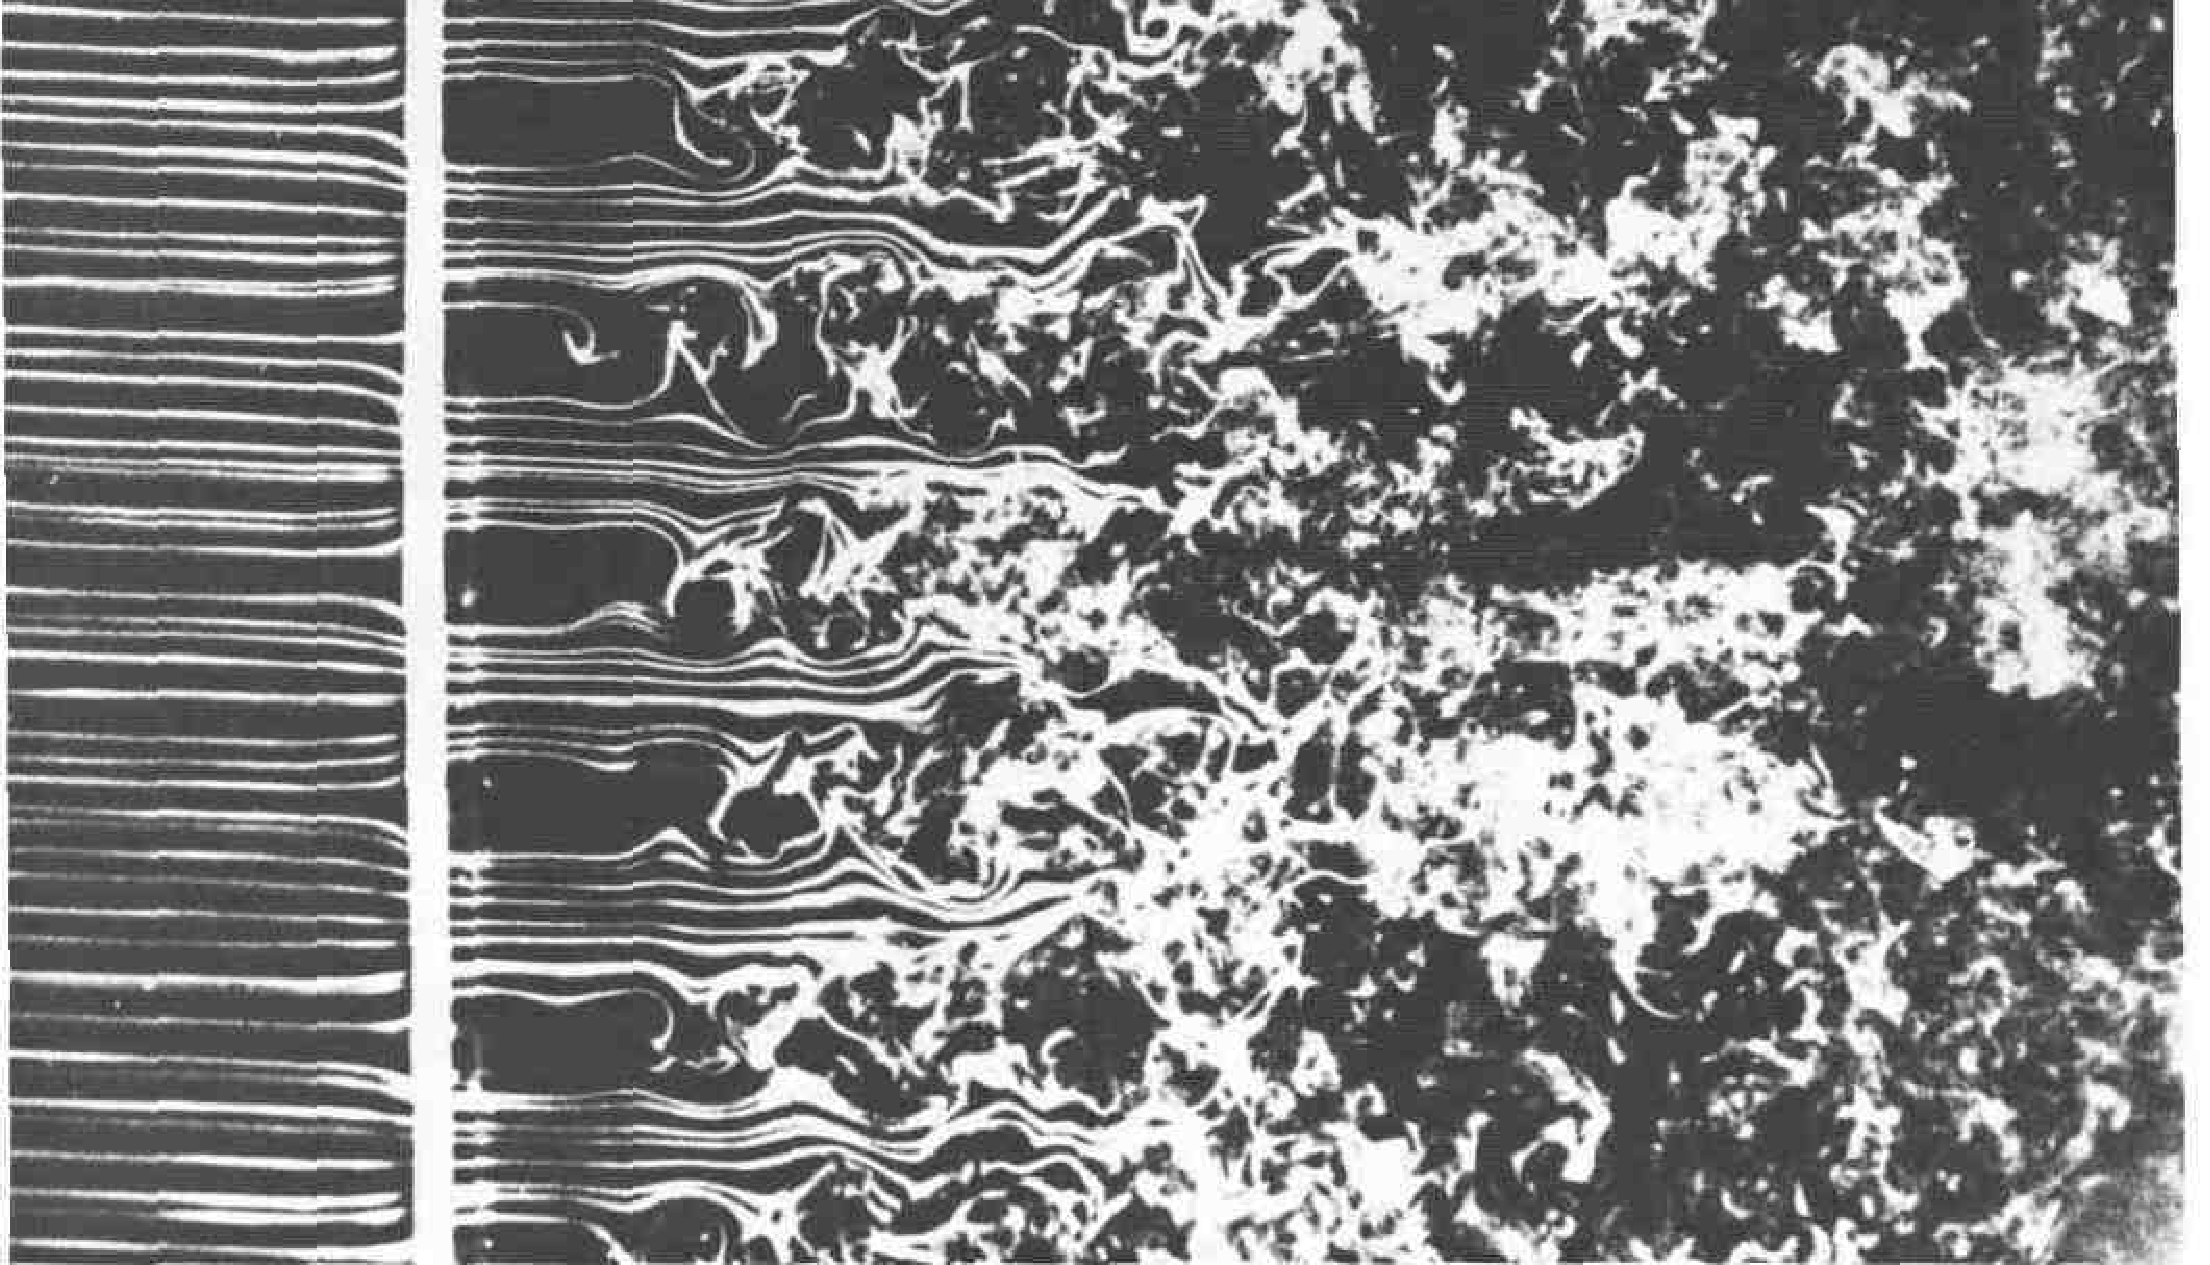
\includegraphics[width=0.7\linewidth]{historyImg/turb.pdf}
\caption{Порождение турбулентности решеткой. Изображние взято с сйта НИИ Мехяники МГУ.}
\label{img:turb}
\end{figure}

Представив скорость $u_i$ в виде суммы средней $\bar u_i$ и пульсационной $u_i'$ составляющих, а давление 
в виде $p=\bar p+p'$, Рейнольдс получил уравнения для средних величин, носящие его имя:
\begin{gather}
\rho\frac{\partial \bar u_j \bar u_i}{\partial x_j} = \frac{\partial}{\partial x_j}\left[ -\bar p \delta_{ij} +
\mu \left ( \frac{\partial \bar u_i}{\partial x_j} + \frac{\partial \bar u_j}{\partial x_i} \right) - 
\rho \overline{ u_i' u_j'} \right]
\label{7}
\end{gather}

Здесь подразумевается суммирование по индексу j. По сравнению с уравнением Навье--Стокса \ref{6} это 
уравнение включает дополнительные напряжения~--- так называемые напряжения Рейнольдса 
$\rho \overline{u_i^\prime u_j^\prime}$. Попытки найти их вид из первых принципов физики оказались безуспешными, 
поэтому уравнение \ref{7} стало базой для развития эмпирических теорий.

К недоопределенной системе \ref{7} следует добавить уравнения для пульсаций и правила осреднения. 
Полученную таким образом расширенную систему уравнений следует называть системой Рейнольдса. Решение 
этой системы кроме среднего и пульсационного слагаемого содержит еще волновой член.

Л.В.~Келлер и А.А.~Фридман дали аналитическую формулировку проблемы турбулентности, сведя задачу к 
бесконечной системе уравнений для статистических моментов. Джеффри Тейлор ввёл в рассмотрение корреляционные 
функции, а также впервые ввёл понятия об однородной и изотропной турбулентности.

Льюис Фри Ричардсон (1881--1953) высказал глубокие соображения о «каскадном процессе» передачи энергии 
по спектру от крупномасштабных мод к мелкомасштабным. Эта картина развитой турбулентности изображена 
Ричардсоном в стихотворении, которое входит во многие учебники по турбулентности:
\begin{center}
Big whorls have little whorls,

Which feed on their velocity;

Little whorls have smaller whorls,

And so on unto viscosity.
\end{center}

Ричардсон любил поэзию. Свою интуитивную теорию турбулентности он создал, вдохновлённый наблюдениями 
за эволюцией облаков.

Парадигма турбулентности ознаменовала превращение гидродинамики из чисто теоретической науки, 
из коллекции оригинальных, но оторванных от жизни решений, в прикладную науку. Разлившаяся река 
стремилась войти в берега актуальной полезности.

Наиболее важным вкладом в теорию турбулентности считаются 4 работы Андрея Николаевича Колмогорова 
(1903--1987), впервые опубликованные в 1941 году. В совокупности они так и называются~--- «теория К 41». 
Колмогоров занимался турбулентностью примерно полгода, до начала войны, а затем, в связи с требованиями 
военного времени, занялся баллистикой. Ещё 2 работы Колмогорова относятся к 1961--1962 годам и называются «теория К 62».

Были ли предшественники у Рейнольдса? Разумеется, каждый человек видел турбулентность в атмосфере, 
в ручье, в струе воды. Хаген ещё в 1839 году установил, что характер течения воды в трубе изменяется 
с увеличением напора. Он считал, что при определённых условиях в потоке возникают внутренние вихри, 
и это приводит к повышению сопротивления, и, следовательно, к уменьшению расхода воды.

Массивным блоком в основании теории турбулентности лежит теория вероятностей, прекрасные исторические 
обзоры которой даны Ширяевым (1998) и Гнеденко (2001). В теории турбулентности есть теория устойчивости 
и перехода ламинарного течения в турбулентное. Рэлею в 1880 году, В.~Орру и А.~Зоммерфельду в 1907--1908 
годах удалось линеаризовать задачу устойчивости в частном случае плоскопараллельного движения. Большое 
значение имеет теория устойчивости пограничного слоя и ламинарно--турбулентного перехода в пограничном слое 
(Бэтчелор, 2000). Следует упомянуть далеко продвинутую теорию изотропной турбулентности (Бэтчелор, 1955).

В XIX веке основной гидродинамической моделью являлась модель идеальной жидкости, в XIX--XX веках~--- 
модель вязкой жидкости. В XXI веке учёные стали вплотную заниматься построением физических и математических
 моделей турбулентности. Следует отметить, что парадигма турбулентности в гидродинамике еще не сформулирована,
  пока видны только её контуры... Построены математические модели случайных процессов в теории броуновского 
  движения и в квантовой механике. Однако построить адекватную модель истории человечества, макроэкономики 
  и турбулентности пока не удалось.

Невозможно провести чёткую границу между гидродинамикой и нелинейной механикой. И там, и там важна нелинейность. 
Актуально как изучение гидродинамических уравнений (Буссинеска, Кортевега--де Вриза и прочих), так и решение 
уравнений нелинейной механики (Шрёдингера, Гинзбурга--Ландау, Синус--Гордона и прочих), которые находят важные 
применения в гидродинамике.

Выдающийся физик Вернер Гейзенберг (1901--1976), серьёзно занимавшийся проблемой турбулентности, признался на 
смертном одре, что хотел бы задать Господу два вопроса~--- об основах теории относительности и о причине 
турбулентности. «Думаю, что Господь ответит мне на первый из них»,~--- галантно заключил он.

% \subsection*{Численное моделирование гидродинамических процессов}

%Усложнение математических моделей привело к тому, что человек перестал справляться с расчетами. Ответом на это  явилось создание компьютера. В то время казалось, что все задачи будут немедленно решены, что восторжествовал принцип пифагорейцев: «Всё есть число». Однако конец эмпирической эпохи в науке и технике не наступил, отодвинувшись на следующее столетие. Современный компьютер позволяет решать сложные задачи гидродинамики, физики плазмы, анализа загрязнения воздуха и грунтовых вод, создания новых лекарств, составления карт озонового слоя, сейсмического анализа. Численные расчёты востребованы как в фундаментальных науках, так и в прикладных.

% Для учёных и инженеров численный расчёт стал обыденным и мощным оружием наступления на непознанное. Численные расчёты практически вытеснили из употребления такие эмпирические методы, как приближения Бубнова--Галёркина в теории пограничного слоя, методы типа Бетца--Мультхопа в теории крыла большого удлинения, полуэмпирические методы в теории турбулентности и так далее. В настоящее время разработаны надёжные методы расчёта ламинарных течений, однако безэмпирический расчёт турбулентных течений пока ещё невозможен. Вычислительная гидродинамика~--- основная часть вычислительной математики, ибо в ней, как ни в одной области физики, задействована нелинейность и, как следствие, турбулентность.

\subsection*{Несколько компьютерных иллюстраций численного моделирования течения жидкости}
\begin{figure}[htp]
\centering
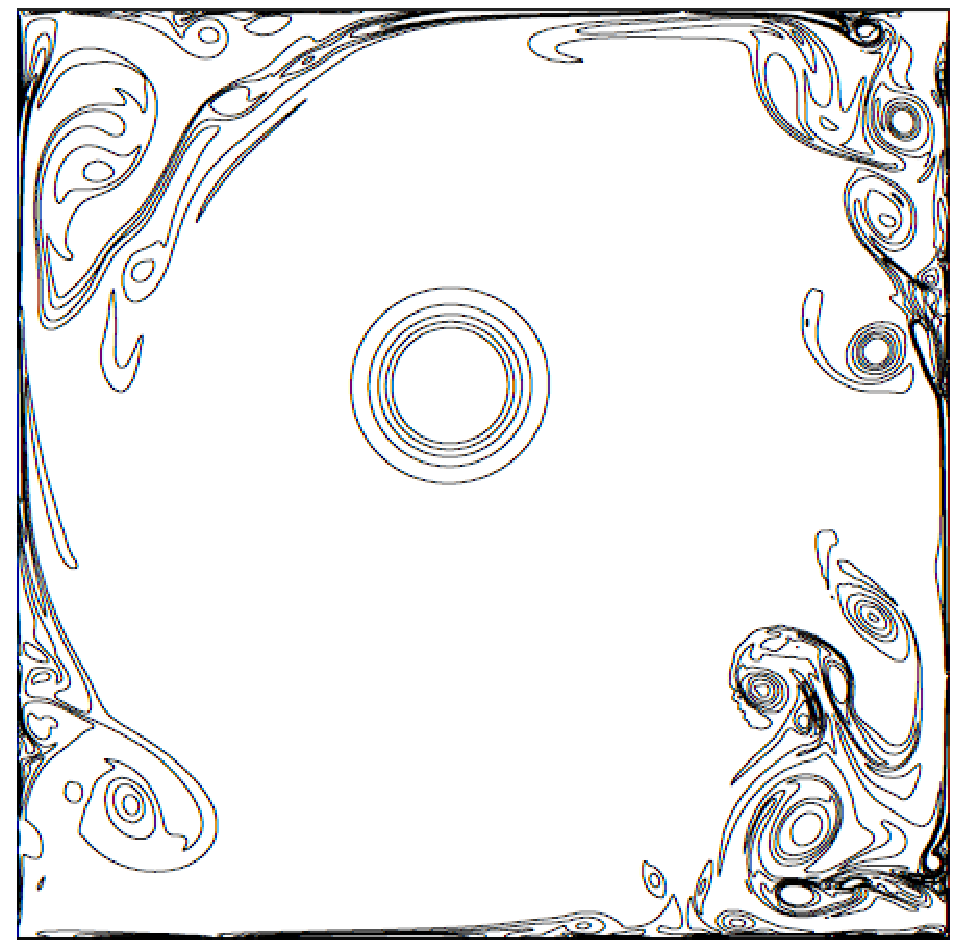
\includegraphics[width=0.7\linewidth]{historyImg/vortex_small.pdf}
\caption{Образование вихрей в вязкой жидкости возое границы из одного начального вихря, смещенного относиткльно центра облости. Покзаны изолини давления:  давление внутри вихря всегда ниже, чем давление снаружи}
\end{figure}

\begin{figure}[htp]
\centering
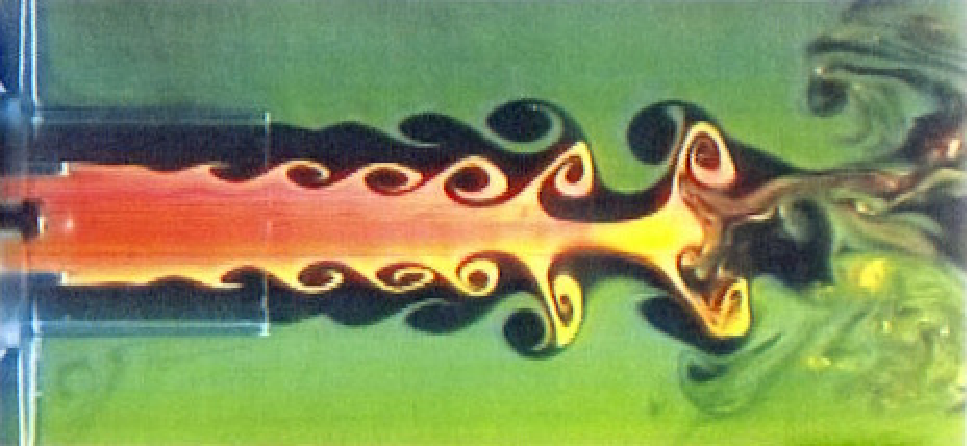
\includegraphics[width = 0.7\linewidth]{historyImg/jet_small.pdf}
\caption{Истечение жидкости из сопла}
\label{}
\end{figure}

\begin{figure}[htp]
\centering
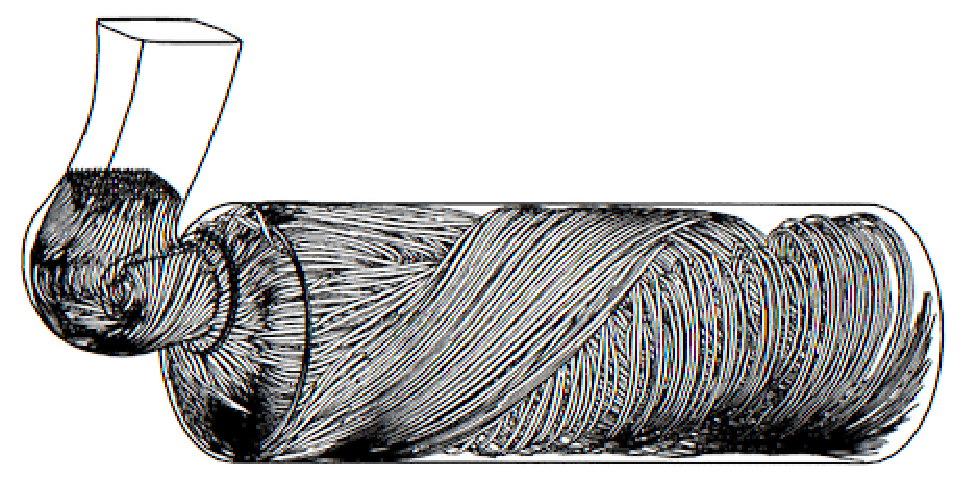
\includegraphics[width=0.7\linewidth]{historyImg/flow_small.pdf}
\caption{<<Нити тока>> жидкости, протекающей через трубу сложной формы}
\label{}
\end{figure}
\newpage

%  \section*{Введение}

С тех пор, как 

%  \section*{Система уравнений Навье-Стокса}


  \section{Математические выкладки}

\subsection{Математическая постановка задачи}

\begin{figure}
  \begin{center}
    \begin{picture}(180,180)(-90,-90)
      \thinlines
      \put(-80,-40){\vector(1,0){160}}
      \put(-40,-80){\vector(0,1){160}}
      %\put(-49,-51){\textsl{0}}
      %\put(37,-51){\textsl{1}}
      %\put(-49,30){\textsl{1}}
      \put(80,-51){\textsl{x}}
      \put(-49,80){\textsl{y}}
      \thicklines
      \put(-40,-40){\line(1,0){80}}
      \put(40,-40){\line(0,1){80}}
      \put(60,40){\line(-1,0){120}}
      \put(60,60){\line(-1,0){120}}
      \put(-40,40){\line(0,-1){80}}
      \put(-60,49.7){\circle{19.5}}
      \put( 60,49.7){\circle{19.5}}
      \put(-10,33){\vector(1,0){30}}
      \put(10,67){\vector(-1,0){30}}
      \thinlines
      \multiput(-40,-40)(0,7){12}{\line(-1,-1){10}}
      \multiput(-40,-40)(7,0){14}{\line(-1,-1){10}}
      \multiput( 40,-44)(0,7){11}{\line(1,1){10}}
      \multiput(-47.5,40)(5,0){20}{\line(0,1){5}}
      \multiput(-47.5,60)(5,0){20}{\line(0,-1){5}}
      \put(53,43){\line(1,1){14}}
      \put(53,57){\line(1,-1){14}}
      \put(-53,43){\line(-1,1){14}}
      \put(-53,57){\line(-1,-1){14}}
    \end{picture}
  \end{center}
  \caption{Каверна с подвижной крышкой}
  \label{pic2D}
\end{figure}

Ставится трехмерная (3D) задача о расчете поля скорости $ \vec v(t) $ в каверне с подвижной крышкой $ \Theta $ . Каверна имеет форму траншеи, бесконечно длинной, с квадратным поперечный сечением $\Theta \times \mathbb{R} \text{, где } \Theta = (0,1) \times (0,1) $. 
Жидкости передается движение крышки $ \Gamma_1 \times \mathbb{R} \text{, где } \Gamma_1 = (0,1) \times {1} $. 
Крышка движется равномерно со скоростью $ \vec{v}_0 = (1,0,0) $. Схематически каверна изображена 
на рисунке \ref{pic2D}. 
Считается, что жидкость вязкая, ньютоновская, несжимаемая, изотермическая, и описывается системой
уравнений Навье-Стокса.
\begin{gather}
  \nabla \cdot \vec v = 0 \label{3D_first}\\
  \frac{\partial \vec v}{\partial t} = \vec v \times \vec \omega - \nabla p - 
  \nu ( \nabla \times \vec \omega ), \text{при } \vec x \in \Theta \times \mathbb{R}\\
  \vec v = (1,0,0), \text{при } \vec x \in \Gamma_1 \times \mathbb{R} \\
  \vec v = (0,0,0), \text{при } \vec x \in \Gamma_2 \times \mathbb{R} \\
  \vec v (0) = \vec v _0 \label{3D_last}
\end{gather}

Здесь $ \vec \omega = \nabla \times \vec v $ - завихренность, p - полное кинематическое давление,
$ \nu = 1 / \Re $ - вязкость, $ \Re $ - число Рейнольдса, $ \Gamma_2 = \partial \Theta \setminus \Gamma_1 $ - боковые стенки и дно каверны, $ \partial \Theta = \Gamma_1 \cup \Gamma_2 $ - 
граница области, $\vec v _0$ - начальное распределение скорости. 

Решение данной задачи \ref{3D_first}\,--\,\ref{3D_last} обозначим как $ \{ \vec V(x,y,z,t), P(x,y,z,t) \} $~--- пара скорость-давление. Тогда $ \{ \vec V(x,y,z), P(x,y,z) \} $~--- стационарное решение этой задачи. 


\subsection{Постановка двумерной задачи}

Хорошо известно, что при достаточно малых числах Рейнольдса в каверне устанавливается двумерное стационарное течение $$ 
  \{\vec V(x,y,z), \vec P(x,y,z) \} = \{[\vec V(x,y), 0], [\vec P(x,y), 0]\}
$$

Здесь $\vec V(x,y)$~--- двумерный вектор скорости, $P(x,y) $~--- давление (скаляр), величины зависят только от двух переменных. Для их нахождения существует двумерная задача, аналогичная задаче \ref{3D_first}\,--\,\ref{3D_last}.
\begin{gather}
  \label{2D_first}
  \nabla \cdot \vec v = 0 \\
  \frac{\partial \vec v}{\partial t} = \vec v \times \vec \omega - \nabla p - 
  \nu ( \nabla \times \vec \omega ), \text{при } \vec x \in \Theta \\
  \vec v = (1,0), \text{при } \vec x \in \Gamma_1\\
  \vec v = (0,0), \text{при } \vec x \in \Gamma_2\\
  \vec v (0) = \vec v _0
  \label{2D_last}
\end{gather}

Здесь вектор $ \vec \omega = \nabla \times \vec v = [0,0,\omega_z]$ имеет компоненту в напралении оси OZ (и только такую компоненту), но в уравнения $ \vec \omega $ входит только в составе выражения $ [(f_x,f_y),0] \times \vec \omega = [(f_y \omega_z, -f_x \omega_z), 0]$, результат которого~--- двумерный вектор, лежащий в плоскости OXY. Систему уравнений \ref{2D_first}\,--\,\ref{2D_last} можно считать двумерной. 

Решение двумерной задачи \ref{2D_first}\,--\,\ref{2D_last} $\{ \vec V, P \}$ далее будет называться \textit{базовым течением}.

\subsection{Линеаризованная система уравнений}

Базовое течение следует проверить на устойчивость к малым трехмерным возмущениям.

Через $\{ \vec v(x,y,z,t), p(x,y,z,t) \} $ обозначены трехмерные \textit{малые возмущения}, наложенные на базовое течение. 
\begin{gather*}
  \vec V(x,y,z,t) = \vec V(x,y) + \vec v(x,y,z,t) \\
  P(x,y,z,t) = P(x,y) + p(x,y,z,t)
\end{gather*}

Новая система уравнений, линейная относительно неизвестных $ \vec v(x,y,z,t)$, $p(x,y,z,t) $, получена путем подстановки выражения в систему уравненй \ref{3D_first}\,--\,\ref{3D_last}. Сокращено принебрежимо малое слагаемое $ \vec v \times \vec \omega $ и использован тот факт, что  $\vec V(x,y), P(x,y) $~--- решение системы \ref{2D_first}\,--\,\ref{2D_last}.
\begin{gather} 
  \label{lin3D_first}
  \nabla \cdot \vec v = 0\\
  \frac{\partial \vec v}{\partial t} = \vec V \times \vec \omega + \vec v \times \vec \Omega - \nabla p - \nu ( \nabla \times \vec \omega ), \text{при } \vec x \in \Theta \times \mathbb{R}\\
  \vec v = (0,0,0), \text{при } \vec x \in \partial \Theta \times \mathbb{R} \\
  \vec v (0) = \vec v _0 \label{lin3D_last}
\end{gather}

Здесь $\vec V = \vec V(x,y) $~--- базовое течение, $ \vec \omega = \nabla \times \vec v $, $ \vec \Omega = \nabla \times \vec V $~--- завихренность малых возмущений и базового течения соответственно, $\vec v_0$~--- распределение малых возмущений в начальный момент времени t=0. 

Над системой уравнений \ref{lin3D_first}\,--\,\ref{lin3D_last} можно выполнить преобразование Фурье по переменной z и перейти от переменной z к волновому числу $\alpha$.

Функции, над которыми было выполнено преобразование Фурье, обозначены соответствующими буквами готического алфавита. Если f(x,y,z)~--- некоторая функция от трех переменных, тогда $ \mathfrak{f}(x,y,\alpha) $~--- соответствующая ей преобразованная функция.
$$
 \mathfrak{f}(x_0,y_0,\alpha) = \int_\mathbb{R} f(x_0,y_0,z) e^{-i\alpha z} dz 
$$

\if 0
Если считать, что $\vec v = (v_x, v_y, v_z)$, $\vec V = (V_x, V_y)$, $\vec \Omega = (0, 0, \Omega_z)$, то в скалярном виде преобразованную систему можно записать так:
\begin{gather} 
  \label{scalar3D_first}
 \frac{\partial \hat v_x}{\partial x} + \frac{\partial \hat v_y}{\partial y} + i\alpha \hat v_z= 0\\
% 
 \frac{\partial \hat v_x}{\partial t} = \vec V \times \vec \omega + \vec v \times \vec \Omega - \nabla p - \nu ( \nabla \times \vec \omega ), \text{при } \vec x \in \Theta \times \mathbb{R}\\
% 
 \frac{\partial \vec v}{\partial t} = \vec V \times \vec \omega + \vec v \times \vec \Omega - \nabla p - \nu ( \nabla \times \vec \omega ), \text{при } \vec x \in \Theta \times \mathbb{R}\\
% 
 \frac{\partial \vec v}{\partial t} = \vec V \times \vec \omega + \vec v \times \vec \Omega - \nabla p - \nu ( \nabla \times \vec \omega ), \text{при } \vec x \in \Theta \times \mathbb{R}\\
% 
 \vec v = (0,0,0), \text{при } \vec x \in \partial \Theta \times \mathbb{R} \\
 \vec v (0) = \vec v _0 
  \label{scalar3D_last}
\end{gather}
\fi

Также введены следующие обозначения для некоторых линейных операторов.
$$
  \nabla_\alpha = (\frac{\partial}{\partial x},\frac{\partial}{\partial y},-\alpha I)\text{,\qquad} 
  \nabla_\alpha^* = (\frac{\partial}{\partial x},\frac{\partial}{\partial y},\alpha I) 
$$

В таких обозначения система уравнений \ref{lin3D_first}\,--\,\ref{lin3D_last}, над которой было выполнено преобразование фурье, имеет вид
\begin{gather} 
  \label{ft3D_first}
  \nabla_\alpha^* \cdot  \mathfrak{\vec v} = 0\\
  \frac{\partial \mathfrak{\vec v}}{\partial t} = \vec V \times \mathfrak{\vec w} + \mathfrak{\vec v} \times \vec \Omega - 
		\nabla_\alpha \mathfrak{p} - \nu ( \nabla \times \mathfrak{\vec w} ), \text{при } \vec x \in \Theta\\
  \vec v = (0,0,0), \text{при } \vec x \in \partial \Theta\\
  \mathfrak{\vec v} (0) = \vec v _0 \label{ft3D_last}
\end{gather}
Здесь $\mathfrak{\vec w} = \nabla_\alpha \mathfrak{\vec v}$ 

\subsection{Решение спектральной задчачи}

Посколько коэффициетны не в системе уравнений \ref{ft3D_first}--\ref{ft3D_last} не зависят от времени, ей можно сопоставить задачу на собственные значения
\begin{gather} 
  \label{s3D_first}
  \nabla_\alpha^* \cdot  \mathfrak{\vec v} = 0\\
  - \lambda \mathfrak{\vec v} = \vec V \times \mathfrak{\vec w} + \mathfrak{\vec v} \times \vec \Omega - 
		\nabla_\alpha \mathfrak{p} - \nu ( \nabla \times \mathfrak{\vec w} ), \text{при } \vec x \in \Theta\\
  \vec v = (0,0,0), \text{при } \vec x \in \partial \Theta\\
  \mathfrak{\vec v} (0) = \vec v _0 \label{s3D_last}
\end{gather}


Спектральная задача \ref{s3D_first}--\ref{s3D_last} зависит от двух параметров. Это число Рейнольдса Re и волновое число $\alpha$. Для каждой пары (Re,$\alpha$) может быть вычислен спектр задачи $\Lambda(\Re,\alpha)$. Декрементом затухания d(Ra,$\alpha$) называтеся наименьшая из действительных частей собственных значений в спектре.
\begin{gather}
 d(\Re,\alpha) = \min_{\lambda \in \Lambda(\Re,\alpha)} \mathfrak{R}(\lambda)
\end{gather}
Здесь $\mathfrak{R}(c)$ обозначает действительную часть числа c. Пусть декременту соответствует множество собственных чисел $\Lambda_d$:
\begin{gather}
 \Lambda_d(\Re,\alpha) = \{ \lambda \in \Lambda(\Re,\alpha) \mid d = \mathfrak{R}(\lambda) \}
\end{gather}
Вообще говоря, множество $\Lambda_d$ включающее только один элемент.
Составим еще одно множество $V_d$ из собственных векторов, соотвтствующих собственным значниям из определенного выше множества. Решение эволюционной задачи можно представить, как линейную комбинацию решений вида 
\begin{gather}
 V_\lambda e^{-\lambda t}
\end{gather}
Здесь $V_\lambda$ - собственный вектор, соответствующий собственному значению $\lambda$. 
По истечении некоторого времени каждым слагаемым, кроме одного, можно будет пренебречь. Останется то слагаемое, собственное значение которого принадлежит множеству $\Lambda_d$. Если d больше нуля, решение устойчиво, если d 
меньше нуля, решение неустойчиво. Если в множестве $\Lambda_d$ всего одно значение $\lambda_d$, то 
решение будет осциллировать с частотой $\frac{\mathfrak{I}(\lambda_d)}{2\pi}$, где 
$\mathfrak{I}(c)$~--- мнимая часть числа c. Значния $d, V_d, \mathfrak{I}(\lambda_d)$ можно найти 
прямым численным интегрированием задачи \ref{lin3D_first}--\ref{lin3D_last}, не решая задачи на собственные значения.



Для каждого $\alpha$ можно вычислить критическое число Рейнольдса, обозначаемое $\Re_{crit}$, как наименьшее число Рейнольдса, при котором задача теряет устойчивость к возмущениям с длиной волны $\alpha$.
\begin{gather}
 \Re_{crit}(\alpha) = inf\{Re>0 \mid d(\Re,\alpha) < 0\}
\end{gather}
Кривую Re$_{crit}(\alpha)$ назовем \textit{кривой нейтральной устойчивости}. Она определена на плоскости $(\Re,\alpha)$ при $\alpha > 0$. Во всех точках, лежащих ниже кривой,~--- задача устойчива к малым возмущениям. 

В реальном мире возмущения развиваются произвольно. Это значит, что в разложении решения по базису из собственных векторов будет присутствовать каждое слагаемое с ненулевым коэффициентом. 
\textit{Глобальное критическое число Рейнольдса} $\Re_{crit}^*$, параметр исследуемой формы каверны, вычисляется как глобальный минимум кривой нейтральной устойчивости. Если при некотором числе Рейнольдса хотя бы при одном значении волнового числа возмущения нарастают, то есть декремент отрицательный, течение неустойчиво к возмущениям. Если $R^+$~--- множество положительных чисел, то
\begin{gather}
 \Re_{crit}^* = \min_{\alpha \in R^+}(\Re_{crit}(\alpha))
\end{gather}



  \section{Численный метод}

\subsection{Аппроксимация трехмерной системы уравнений}

Для аппроксимации как двумерной задачи, так и линеаризованных уравнений применен метод\cite{method}, поэтому здесь представлен способ аппроксимиции трехмерной системы уравнений как более общий случай.

В работе применен конечно--разностный метод, позволяющий найти решение со вторым порядком точности по пространству и с третьим порядком точности по времени. В расчетной области вводится разнесенная неравномерная сетка. Метод применим только в том случае, когда в области можно ввести ортогональную систему координат, в которой область представляет из себя параллелепипед со стенками, параллельными координатным осям. То есть, если $\Omega$~--- расчетная область, то существуют такие отрезки $l_1, l_2, l_3$, что $\Omega = l_1 \times l_2 \times l_3$. 

\begin{figure}[htp]
  \begin{center}
    \begin{picture}(180,180)(-90,-90)
      \thinlines
     \put(-90,10){\vector(0,1){40}}
     \put(-90,10){\vector(1,0){40}}
     \put(-90,10){\vector(-1,-1){20}}
     \put(-97,46){\text{z}}
     \put(-56,3){\text{y}}
     \put(-110,-2){\text{x}}
      \thicklines
     \put(-30,-30){\line(0,1){60}}
     \put(-30,30){\line(1,0){60}}
     \put(30,30){\line(0,-1){60}}
     \put(30,-30){\line(-1,0){60}}
     %
     \put(-30,30){\line(1,1){24}}
     \put(30,30){\line(1,1){24}}
     \put(30,-30){\line(1,1){24}}
     %
     \put(-6,54){\line(1,0){60}}
     \put(54,54){\line(0,-1){60}}
      \thinlines
%     \put(-30,-30){\line(1,1){24}}
%    \put(-6,-6){\line(1,0){60}}
%     \put(-6,-6){\line(0,1){60}}
      \thicklines
     \put(0,0){\circle{6}}
     \put(3,-7){\text{$v_x$}}
     \put(42,12){\circle{6}}
     \put(44,5){\text{$v_y$}}
     \put(12,42){\circle{6}}
     \put(15,35){\text{$v_z$}}
     \put(-30,0){\circle*{4}}
     \put(-27,-7){\text{$\omega_z$}}
     \put(0,30){\circle*{4}}
     \put(3,23){\text{$\omega_y$}}
     \put(0,-30){\circle*{4}}
     \put(3,-37){\text{$\omega_y$}}
     \put(30,0){\circle*{4}}
     \put(33,-7){\text{$\omega_z$}}
     \put(54,24){\circle*{4}}
     \put(57,17){\text{$\omega_z$}}
     \put(42,-18){\circle*{4}}
     \put(45,-25){\text{$\omega_x$}}
     \put(42,42){\circle*{4}}
     \put(43,35){\text{$\omega_x$}}
     \put(24,54){\circle*{4}}
     \put(27,47){\text{$\omega_y$}}
     \put(-18,42){\circle*{4}}
     \put(-15,35){\text{$\omega_x$}}
    \end{picture}
  \end{center}
  \caption{Расположение узлов, к которым относятся компоненты векторов скорости и завихренности, на смещенных сетках. Изображена одна ячейка сетки. Давление p определяется в центре ячейки.}
  \label{picStag}
\end{figure}


Для того чтобы ввести неравномерную сетку, используется непрерывная монотонная функция преобразования $ x = x(\xi) $  , отображающая отрезок [0,1] в отрезок [0,1]. 
\begin{gather}
  x(\xi): [0,1] \longrightarrow [0,1]
\end{gather}
Такая функция переведет одномерную равномерную сетку, введеную на отрезке [0,1] в неравномерную. Введем равномерную сетку из $N_x$ ячеек 
\begin{gather}
 \Xi = \{\xi_i = ih, i = \overline{0..N_x}\}, \qquad h = 1 / N_x 
\end{gather}
Под разностной схемой, построенной на разнесенных сетках\footnote{так же разнесенными сетками называют перемежающиеся сетки, или смещенные сетки, Angl.: staggered mash.}, понимают такую, в которой разные неизвестные величины определены в разных узлах. В нашем случае одни неизвестные относятся к узлам сетки, то есть определены на множестве $\Xi$, а другие относятся к центрам ячеек, и определены соответственно на множестве $\Xi_f$
\begin{gather}
 \Xi_f = \{ \xi_i = i*h - h/2, i = \overline{1..N_x} \}, \qquad h = 1/N_x
\end{gather}
Неравномерные сетки $X$ и $X_f$ есть отображение сеток $x(\xi)$ на $\Xi$ под действием преобразования $x(\xi)$
\begin{gather}
 X = x(\Xi) = \{x_i = x(\xi_i), \xi_i \in \Xi\} \\
 X_f = x(\Xi_f) = \{ x_i = x(\xi_i), \xi_i \in \Xi_f \}
\end{gather}

Если переменная определена в центрах ячеек, ее индекс соответствует номеру ячейки и меняется от 1 до $N_x$, а если переменная определена в узлах сетки, ее индекс соответствует номеру узла и меняется от 0 до $N_x$.

Далее используется обозначение $f_i = f(x_i) = f(x(\xi_i))$~--- значение неизвестной переменной f в i-ой точке сетки. Если сказано, что переменная относится к центру ячейки, то она определена на сетке $\Xi_f$.  

Для произвольной функции f(x) справедливо утверждение:
$$
  \frac{\partial f}{\partial x} = \frac{\partial f}{\partial \xi} \frac{\partial \xi}{\partial x}
$$
Значение производной функции $x(\xi)$ может быть вычислено точно, так как явный вид функции известен.
В соответствии с данным утверждением построен разностный оператор дифференцирования $\delta_x$, аппроксимирующий производную со вторым порядком точности
\begin{gather}
 \delta_x f_i = \frac{\partial x(\xi_i)}{\partial \xi} \frac{f(x(\xi_i + h/2)) - f(x(\xi_i - h/2))}{h}  = \frac{\partial f(x_i)}{\partial x} + O(h^2)
\end{gather}

В частном случае, если предположить, что переменная $f$ определена в узлах сетки $ f_i \in F = f(X)$, то $\delta_x f$ относится к центрам ячеек и определяется выражением
$$
  (\delta_x f)_i = (f_i - f_{i-1}) \Delta_i, \text{ где } \Delta_i =  \frac{1}{h}\frac{\partial x(h*i - h/2)}{\partial \xi}
$$

Если, наоборот, $f$ определена в центрах ячеек $ f_i \in F = f(X_f)$, тогда $\delta_x f$
относится к узлам сетки и определяется выражением
$$
  (\delta_x f)_i = (f_{i+1} - f_i) \Delta_i, \text{ где } \Delta_i  = \frac{1}{h}\frac{\partial x(h*i)}{\partial \xi}
$$

Так же вводится выражение для осреднения по пространству произвольной функции f(x) со вторым порядком точности. Оператор осреднения обозначается горизонтальной чертой над функцией. 
$$
  \overline{f}^x_i = \frac{f(x(\xi_i - h/2)) + f(x(\xi_i + h/2))}{2} = f_i + O(h^2)
$$

В нашем случае, если $f$ определена в узлах сетки $f_i \in F = f(X)$, тогда $\overline{f}^x_i$ относится к центрам ячеек и определяется выражением
$$
  \overline{f}^x_i = \frac{f_{i-1} + f_{i}}{2}
$$

Если $f$ определена в центрах ячеек $f_i \in F = f(X_f)$, тогда $\overline{f}^x_i$ относится к узлам сетки и определяется выражением
$$
  \overline{f}^x_i = \frac{f_i + f_{i+1}}{2}
$$


Далее описано введение сетки в трехмерной области. 
По аналогии с парой $\{X,X_f\}$, введены пары сеток $\{Y,Y_f\}$ и $\{Z,Z_f\}$. В нашем случае необходимо вычислить три компоненты вектора скорости, три компоненты вектора завихренности и давление. Давление относится к центрам ячеек. Это значит, что оно определено на множестве точек $X_f \times Y_f \times Z_f$.
$$
  P = \{p_{ijk} = p(x_i,y_j,z_k), \text{ при } x_i \in X_f, y_i \in Y_f, z_i \in Z_f\}
$$
Компоненты вектора скорости относятся к центрам граней ячеек, вектор нормали которых сонаправлен с определяемым вектором.
\begin{gather*}
  V_x = \{ v^x_{ijk} = v_x(x_i,y_j,z_k), \text{ при } x_i \in X, y_i \in Y_f, z_i \in Z_f \} \\
  V_y = \{ v^y_{ijk} = v_y(x_i,y_j,z_k), \text{ при } x_i \in X_f, y_i \in Y, z_i \in Z_f \} \\
  V_z = \{ v^z_{ijk} = v_z(x_i,y_j,z_k), \text{ при } x_i \in X, y_i \in Y_f, z_i \in Z \}
\end{gather*}
Компоненты вектора завихренности определяются в центрах ребер ячейки, сонаправленных с определяемым вектором. 
\begin{gather*}
  \Omega_x = \{ \omega^x_{ijk} = \omega_x(x_i,y_j,z_k), \text{ при } x_i \in X_f, y_i \in Y, z_i \in Z \} \\
  \Omega_y = \{ \omega^y_{ijk} = \omega_y(x_i,y_j,z_k), \text{ при } x_i \in X, y_i \in Y_f, z_i \in Z \} \\
  \Omega_z = \{ \omega^z_{ijk} = \omega_z(x_i,y_j,z_k), \text{ при } x_i \in X, y_i \in Y, z_i \in Z_f \}
\end{gather*}
Иллюстрация на Рис \ref{picStag}.

Этого достаточно чтобы записать разностную аппроксимацию исходной системы уравнений. Для прямоугольной системы координат, как в нашем случае, разностная аппроксимация системы несколько проще, чем для произвольной ортогональной системы координат, и записывается так:
\begin{gather}
  \delta_x v_x + \delta_y v_y + \delta_z v_z = 0 
  \\
  \omega_x = \delta_y v_z - \delta_z v_y 
  \\
  \omega_y = \delta_z v_x - \delta_x v_z 
  \\
  \omega_z = \delta_x v_y - \delta_y v_x 
  \\
  \frac{\partial v_x}{\partial t} = \frac{1}{y'}\overline{\overline{y'v_y}^x \omega_z}^y - \frac{1}{z'}\overline{\overline{z'v_z}^x \omega_y}^z - \delta_x p - \nu (\delta_y \omega_z - \delta_z \omega_y)
  \\
  \frac{\partial v_y}{\partial t} = \frac{1}{z'}\overline{\overline{z'v_z}^y \omega_x}^z - \frac{1}{x'}\overline{\overline{x'v_x}^y \omega_z}^x - \delta_y p - \nu (\delta_z \omega_x - \delta_x \omega_z) 
  \\
  \frac{\partial v_z}{\partial t} = \frac{1}{x'}\overline{\overline{x'v_x}^z \omega_y}^x - \frac{1}{y'}\overline{\overline{y'v_y}^z \omega_x}^y - \delta_z p - \nu (\delta_x \omega_y - \delta_y \omega_x)
\end{gather}
Зная значение скоростей в каждой точке на каждом шаге и используя приведенные формулы, можно расчитать производную скорости по времени. 

\subsection{Интегрирование по времени}

Решаемая задача~--- задача Каши, для интегрирования по времени применим метод Рунге--Кутта третьего порядка точности.
Если интегрируемую систему представить в виде 
$$
	\dot w = H(t,w),
$$
обозначить за D~--- оператор дивиргенции, G~--- оператор градиента, L - некоторый линейный оператор, то метод представим в следующем виде:

\begin{gather}
\begin{align*}
Step 1:& \\
&&H_n &= H(t_n, w_n) \\
&&DGp_n &= DH_n \\
&&(I - \gamma \tau L)(w' - w_n) &= \frac{2}{3} \tau (H_n - Gp_n) \\
%
Step 2:& \\
&&H' &= H(t_n + 2\tau/3, w') \\
&&DGp' &= DH' \\
&&(I - \gamma \tau L)(w'' - \frac{2}{3}w' + \frac{1}{2}w_n) &= \frac{1}{2} \tau (H' - Gp') + w_n - w' \\
&&(I - \gamma \tau L)(\tilde w_{n+1} - \frac{3}{2}w'' + \frac{3}{4}w' - \frac{1}{4}w_n) &= \frac{3}{4}(w'' - w_n)\\
%
Step 3:& \\
&&H'' &= H(t_n + 2\tau/3, w'') \\
&&(I - \gamma \tau L)(\hat w_{n+1} - \frac{1}{2} \tilde w_{n+1} - \frac{3}{4}w'' + \frac{1}{4}w_n) &= \frac{3}{4} \tau (H'' - Gp') + 
	\frac{5}{8}w_n + \frac{3}{8}w'' - \tilde w_{n+1} \\
&&DGq &= D\tilde w_{n+1} \\
&&w_{n+1} &= \hat w_{n+1} - Gq
\end{align*}
\end{gather}

Если выбрать L = 0, получим явный метод. Но несмотря на нелинейность задачи, выбором оператора L можно увеличить область сходимости метода. Такой метод называется \textit{полунеявным}\footnote{Англ: semi-implicit}. 

Оптимальное значение параметра $\gamma$ выбирается эмпирическим путем, при расчетах был выбран $\gamma=0.5$. 

Замечено, что причина неустойчивости численного метода лежит в слагаемом, отвечающем за вязкость$$
	\nu (\nabla \times \vec \omega) = \nu \nabla ^2 \vec v
$$ Это линейный оператор, поэтому можно выбрать $L = \nu \nabla^2$. Здесь $\nu = \frac{1}{Re}$~--- кинематическая вязкость. 

На практике удобнее модифицировать оператор L так, чтобы выполнялось соотношение
\begin{gather*}
	(I - \gamma \tau L) = (I - \gamma \tau \nu \delta_x^2)(I - \gamma \tau \nu \delta_y^2) \\
	L =  \nu (\delta_x^2 + \delta_y^2) - \gamma \tau \nu \delta_x^2 \delta_y^2 = \nu \nabla^2 + o(\tau)
\end{gather*}
С одной стороны, оператор L приближает вязкий член уравнения с первым порядком малости $\tau$, с другой стороны, неявное уравнение можно решить, применив прогонку по каждому из направлений. Время, затраченое на прогонку, несравнимо мало по сравнению с временем, требуемым на решение эллиптического уравнения для давления. 

Выбрав таким образом оператор L, можно при Re=1000, например, увеличить область устойчивости на два порядка, то есть уменьшить время счета также на два порядка, что весьма существенно. 




%  \section*{Программная реализация}

  \section*{Результаты} 

Спектральная задача \ref{spactralProblem} зависит от двух параметров. Это число Рейнольдса Re и волновое чисо $\alpha$. Для каждой пары (Re,$\alpha$) может быть вычислен спектр задачи $\sigma(\Re,\alpha)$. Вычислив действительную часть каждого собственного значения в спектре и найдя среди них наименьшую найдем декримент затухания d(Ra,$\alpha$)
\begin{gather}
 d(\Re,\alpha) = \min_{\lambda \in \sigma(\Re,\alpha)} \mathfrak{R}(\lambda)
\end{gather}
Здесь $\mathfrak{R}$ обозначает реальную часть числа. Пусть дикременту соответствует множество собственных чисел $\Lambda_d$, вообще говоря, включающее только один элемент.
\begin{gather}
 \Lambda_d(\Re,\alpha) = \{ \lambda \in \sigma(\Re,\alpha) \mid d = \mathfrak{R}(\lambda) \}
\end{gather}
Составим еще одно множество $V_d$ из собственных векторов, соотвтствующих собственным значниям из определенного выше множества. Решение эволюционной задачи можно представить, как линейную комбинацию решений виде 
\begin{gather}
 V_\lambda e^{-\lambda t}
\end{gather}
Здесь $V_\lambda$ - собственный вектор, соответствующий собственному значению $\lambda$. 
По истечению некоторого времени каждым слагаемым, кроме того, собственное значение которого из
множества $\Lambda_d$, можно будет принебрачь. Если d больше нуля, решения устойчево, если d 
меньше нуля, решение неустойчево. Если в множестве $\Lambda_d$ всего одно значение $\lambda_d$, то 
решение будет асцелировать с частотой $\frac{\mathfrak{I}(\lambda_d)}{2\pi}$, где 
$\mathfrak{I}$~--- мнимая часть числа. Значния $d, V_d, \mathfrak{I}(\lambda_d)$ можно найти 
прямым численным интегрирование задачи \ref{iii}, не решая задачи на собственные значения.



Для каждого $\alpha$ можно вычислить критическое число Рейнольдся, обозначаемое $\Re_{crit}$, как наименьшее число Рейнольдся, при котором задача теряет устойчивость к возмущениям с длиной волны $\alpha$.
\begin{gather}
 \Re_{crit}(\alpha) = inf\{Re>0 \mid d(\Re,\alpha) < 0\}
\end{gather}
Кривую Re$_{crit}(\alpha)$ назавем \textit{кривой нейтральной стабильности}. Она определна на плоскости $(\Re,\alpha)$ при $\alpha > 0$. Во всех точках, лежищих ниже кривой,~--- задача устойчива к малым возмущениям. 

Расчет проводился при значениях числа рейнольдса от 100 до 5000, изменяющегося с шагом 50, и значениях волнового числа от 1 до 20, изменяющихся с шагом 1. Если решать задачу при каждом значении числа Рейнольдса и волнового числа, всего нужно провести 2000 испытвний. Для того, что бы число испытаний уменьшить, был использован следующий алгоритм. Для нахождения $Re_{crit}(\alpha)$ используется значение $\Re_{crit}(\alpha - \Delta\alpha)$. Вычисляется $d = d(\Re_{crit}(\alpha - \Delta\alpha), \alpha)$ если d > 0, вычисляем новое значение d при увеличеном на $\Delta \Re$ числе ренольдся, если d < 0~--- уменьшаем Re на $\Delta \Re$. Так, пока не будет найдено новое критическое сило рейнольдся. 
Таким образом можно сократить число испытвний, примерно, до 60. 

Численное решение спектральной задачи требует большого объема памяти и уже на сетках $50 \times 50$ памяти персонального компьютера не достаточно для расчета. Такой сетки достаточно лишь для чисел Рейнольдса, меньших 150. Для других чисел Рейнольдса, когда решить спектральную задачу не представляется возможным, линеаризованная система уравнений \ref{} интегрируется по времени до установления коэфициента затухания к значению дикремента. Так же, при Re < 150, результаты, полученный прямым численным интегрированием и из решения спектрильной задачи, можно сравить для проверки правельности програмной реализации и теоретических выкладок, что было успешно сделано. 
В таблтце \ref{Re_al} представленны результаты расчета в старвнении с результатами, получанными в \cite{lin-stability}. При $\alpha = 15$ значение $\Re_{crit}$ было вычисленно более точно, как как в этой точке достигается манимум.

\begin{table}
 \begin{tabular}{cccccc}
\hline
\hline
  \multicolumn{3}{c}{Бифуркация Андронова--Хопфа} & \multicolumn{3}{c}{Стационарные бифуркации} \\
  $\alpha$&	$\Re_{crit}(\alpha)$ \cite{lin-stability}&  Пр.&	$\alpha$&	$\Re_{crit}(\alpha)$ \cite{lin-stability}&  Пр. \\
\hline
  1&	8047&		-&	12&	925&		950\\ 
  2&	8046.6&		-&	13&	837.69&		850\\
  3&	4772.68&	4800&	14&	799.3&		800\\
  4&	4769.25&	4800&	15&	786&		785\\
  5&	1967.9&		1950&	16&	786&		800\\
  6&	1032&		1050&	17&	795.74&		800\\
  7&	932.5&		950&	18&	811.92&		850\\
  8&	939&		950&	19&	832.58&		850\\
  9&	1029.8&		1050&	20&	856&		900\\
  10&	1132&		1150\\
  11&	1040&		1050\\
\hline
 \end{tabular}
 \caption{Зависимость критического числа Рейнольдса от волнового числа. Для сравнения приведено решение из \cite{lin-stability}. }
 \label{Re_al}
\end{table}

\begin{figure}
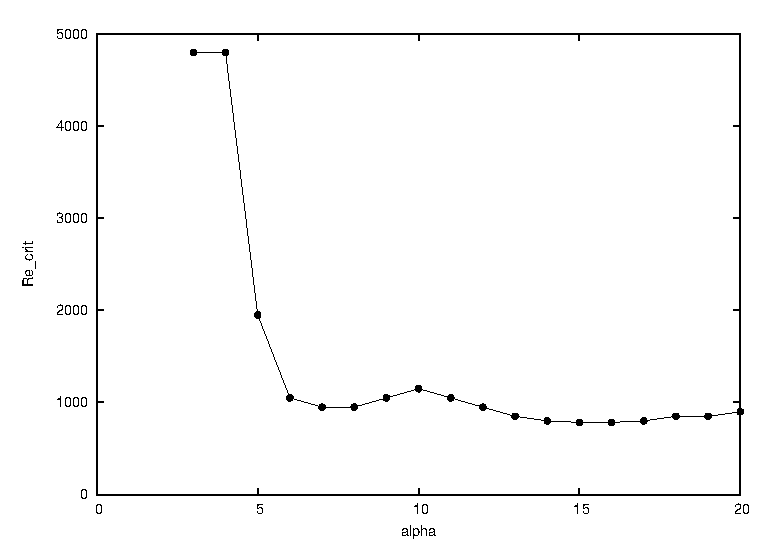
\includegraphics{Re}
\caption{Кривая нейтральной устойчивости}
\label{img:Re_al}
\end{figure}


\newpage

\section*{Заключение}
	Была написана программа для решения двумерных уравнений Навье-Стокса. С ее помощью были вычислены стационарные течения в квадратной каверне с подвижной крышкой для случая, когда крышка движется с постояной скоростью, при некоторых числах Рейнольдса. Полученные стацонарные течения были исследованы на устойчивость к малым трехмерным возмущениям в рамках линеаризованной системы уравнений. Для этого была написана программа, решающая соответствующую собственную задачу, и программа для прямого интегрирования малых возмущений по времени. Программа была написана с использованием технологии MPI, и расчеты были проведены на суперкомпьютере МГУ "Чебышев". Был определен декремент затухания при некоторых волновых числах и некоторых числах Рейнольдса, найдена кривая нейтральной устойчивости и пороговое число Рейнольдса, при котором двумерное течение теряет устойчивость к малым трехмерным возмущениям. Это пороговое значение числа Рейнольдса составляет 790. Было продемонстрировано хорошее соответствие полученных результатов результатам других авторов. Достоинствами использованного метода являются простота реализации, возможность получить хороший результат на достаточно грубых сетках. 


В будущем можно продолжить работу, исследовав характер неустойчивости более детально. При числе Рейнольдса из некоторой окрестности критического числа Рейнольдса определить собственный вектор, соответствующий главному собственному значению, и восстановить форму течения, в котором нарастают возмущения. Найти причину возникновения неустойчивости. 
Провести то же исследование в кавернах других форм. Изменить характер движения крышки. Добавить учет новых физических явлений, таких как температура или электростатические силы. Написать программу для решения трехмерной системы уравнений Навье-Стокса. Найти устойчивые решения задачи при надкритических числах Рейнольдса. Определить возможные устойчивые решения при докритических числах Рейнольдса. 

  \begin{thebibliography}{99}

  \bibitem{method}
  \textit{N.\,Nikitin}, Finite-difference method for incompressible Navier–Stokes equations in 
  arbitrary orthogonal curvilinear coordinates // J. Comput. Phys. 217 (2006) 759–781.

  \bibitem{lin-stability}
  \textit{Etienne Non, Roger Pierre, and Jean-Jacques Gervais}, Linear stability of the 
  three-dimensional lid-driven cavity // Physics of Fluids 18, 084103 (2006)
  
  \bibitem{introduction}
   \textit{Ramanan\.N., Homsy\.G.\.M.} Linear stability of lid-driven cavity flow 
  //Physics of Fluids.~--- 1994.~--- Т. 6.~--- С. 2690.
  
  \bibitem{2DBench}
   \textit{Erturk\.E., Corke\.T.\.C., Gökçöl\.C.} Numerical solutions of 2-D steady incompressible
  driven cavity flow at high Reynolds numbers //International Journal for Numerical Methods in 
  Fluids.~--- 2005.~--- Т. 48.~--- №. 7.~--- С. 747--774.

	\bibitem{KimMoin}
	\textit{J.~Kim and P.~Moin}, Application of a fractional step method to incompressible Navier-Stokes equations//
 J.~Comput.~Phys. 59, 308 (1985).

  \bibitem{betyaev}
   \textit{Бетяев~С.К.} Пролегомены к // РХД, 2006 г. 304 стр
  
  \bibitem{wiki}
   Материал из Википедии~--- свободной энциклопедии [ru.wikipedia.org]

  \bibitem{history}
   История гидродинамики, опубликованно 29-го января 2009 г [http://iproc.ru/interesting/hydro-history]

\end{thebibliography}

\end{document}
